\documentclass{ximera}
\graphicspath{     %% setup a global graphics path
{./}               %% look in the same-level directory
{./pictures/}      %% look in graphics
{../pictures/}     %% look up one directory, then in graphics
%{../../pictures/} %% look up two directories, then in graphics
}

\author{Zack Reed}
%borrowed from selinger linear algebra
\title{Describing Eigenvalues and Eigenvectors}
\begin{document}
\begin{abstract}

\end{abstract}
\maketitle


\section*{Describing Eigenvalues and Eigenvectors}

    
At several places so far, it has been valuable to restrict ourselves to square matrices, and we do so again when discussing eigenvalues and eigenvectors. 
    
Recall that any $n \times n$  matrix is a linear transformation from $\RR^n$ to itself.  For our first few examples, let us consider the case $n = 2$.
    
\begin{exploration}\label{init:eignintro}
Let $A=\begin{bmatrix} 2& 1\\ 1&2
\end{bmatrix}$. Re-familirize yourself with the \emph{linear transformation} interpretation of a matrix by using the following GeoGebra applet to visualize the transformation of space onset by a matrix as well as the image of any selected vector. 

\begin{center}
    \geogebra{fxktu8e2}{1073}{592}
\end{center}
    
    For many vectors, $A\vec{x}$ does not point in the same direction as $\vec{x}$. If you slowly rotate $\vec{v}$ around the origin, however, you will find that four vectors point in the exact same direction as their image vector $A\vec{v}$.

    Try it out for other matrices as well and ask yourself: in addition to pointing in the same (or opposite) direction as $\vec{v}$, does $A\vec{v}$ grow, or shrink, or flip orientation? These are the questions that specifically involve a special collection of vectors called \emph{eigenvectors}.
    

\end{exploration}
    
In Exploration \ref{init:eignintro} we found that certain vectors do not change direction under the linear transformation induced by matrix $A$.  Such vectors are examples of \textbf{eigenvectors} of $A$.
    
In general, any nonzero vector whose image under a matrix transformation is parallel to the original vector is called an \dfn{eigenvector} of the matrix that induced the transformation.  The following definition captures this idea algebraically.
    
\begin{definition}\label{def:eigen}

Let $A$ be an $n \times n$ matrix.  We say that a non-zero vector $\vec{x}$ is an \dfn{eigenvector} of $A$ if $$A\vec{x} = \lambda \vec{x}$$
for some scalar $\lambda$.
We say that $\lambda$ is an \dfn{eigenvalue} of $A$ associated with the eigenvector $\vec{x}$. 
\end{definition}

Here's a video by Grant Sanderson providing a very effective visual exploration of the main ideas of eigenvalues and eigenvectors that we'll be focusing on in this chapter. The very end of the video dips into content for next chapter, involving diagonalization and changes of bases, so for now feel free to only pay attention to the video until around 13:02. The whole video might be nice to get a look at what comes next, but the final 4 minutes is technically not necessary.

\begin{center}
    \youtube{PFDu9oVAE-g?si=a6C_O0_jfXJk8Z32}
\end{center}
    
Let's revisit Exploration \ref{init:eignintro} in light of Definition \ref{def:eigen}.  In the exploration, we observed visually that vectors parallel to $\begin{bmatrix} 1\\ 1 \end{bmatrix}$ were eigenvectors associated with $A=\begin{bmatrix} 2& 1\\ 1&2
\end{bmatrix}$, as these vectors changed length but remained parallel to the original vector under the linear transformation induced by $A$.  To verify this algebraically, observe that all vectors parallel to $\begin{bmatrix} 1\\ 1 \end{bmatrix}$ can be written in the form $\begin{bmatrix} a\\ a \end{bmatrix}$, $(a\neq 0)$.  We compute
$$\begin{bmatrix} 2& 1\\ 1&2 \end{bmatrix} \begin{bmatrix} a\\ a \end{bmatrix} =
\begin{bmatrix} 3a\\ 3a \end{bmatrix}= 3 \begin{bmatrix} a\\ a \end{bmatrix}$$
This shows that any non-zero scalar multiple of $\vec{v}=\begin{bmatrix} 1\\ 1 \end{bmatrix}$ is an eigenvector of $A$ which has a corresponding eigenvalue of 3.
    
\begin{center}
    %make the scale 1.2
\begin{tikzpicture}[scale=1.2]
    
    \draw[<->] (-4,0)--(4,0);
    \draw[<->] (0,-4)--(0,4);
    
    \draw[line width=1pt,-stealth, blue](0, 0)--(1, 1);
    \draw[line width=1pt,-stealth, blue](0, 0)--(2, 2);
    \draw[line width=1pt,-stealth, blue](0, 0)--(3, 3);
    \draw[line width=1pt,-stealth, blue](0, 0)--(-1, -1); 
    \draw[line width=1pt,-stealth, blue](0, 0)--(-2, -2);
    \draw[line width=1pt,-stealth, blue](0, 0)--(-3, -3);
    
    
    \node[blue] at (3, 3.5)   (a) {$A*\vec{v}=3\vec{v}$};
    
    \end{tikzpicture}
\end{center}
    
\dfn{Fixed vectors} of Exploration \ref{init:eignintro} are also eigenvectors.
For example, 
$$\begin{bmatrix} 2& 1\\ 1&2 \end{bmatrix} \begin{bmatrix} 1\\ -1 \end{bmatrix} =
\begin{bmatrix} 1\\ -1 \end{bmatrix}= 1 \begin{bmatrix} 1\\ -1 \end{bmatrix}$$
This shows that $\begin{bmatrix} 1\\ -1 \end{bmatrix}$ is a fixed vector and an eigenvector of $A$ which has a corresponding eigenvalue of $1$.
    
The above discussion leads us to the following result.
    
\begin{theorem}\label{th:eigenScalarMult}
    If $\vec{x}$ is an eigenvector of matrix $A$ and $\lambda$ is the corresponding eigenvalue, then every scalar multiple of $\vec{x}$ is also an eigenvector of $A$
    and $\lambda$ is the corresponding eigenvalue.
\end{theorem}
\begin{proof}

\end{proof}
    
\begin{observation}\label{obs:finerPointsOfEigDef}
A couple of finer points of Definition \ref{def:eigen} require clarification.
    \begin{itemize}
    \item We require eigenvectors to be non-zero.  
    
    Imagine what would happen if we allowed $\vec{x}=\vec{0}$ to be an eigenvector of $A$. Clearly $A\vec{0}=\lambda\vec{0}$ for all scalars $\lambda$.  This means that every number would be an eigenvalue of every matrix.  Because eigenvalues are supposed to capture certain information about the matrix, allowing every number to be an eigenvalue of every matrix would defeat the purpose.
    \item Until now, we had talked about  eigenvectors as vectors whose images under a matrix transformation are parallel to the original vectors.  
    
    But the algebraic definition allows non-zero vectors that map to zero to be considered eigenvectors.  (What would an eigenvalue of such an eigenvector be?)  The zero vector has no direction, so we cannot say that the image of such an eigenvector is parallel to the original vector.  Example \ref{ex:eigen} will illustrate this point.
    \end{itemize}
\end{observation}
    
\begin{example}\label{ex:eigen}
Let $P=\begin{bmatrix} 1& 0\\ 0&0\end{bmatrix}$.  Note that $P$ takes a vector in $\RR^2$ and projects it onto the $x$-axis.

Which vectors in $\RR^2$ would be the eigenvectors, and what are the corresponding eigenvalues?
\begin{explanation}
Since $P\vec{x}$ is the projection of $\vec{x}$ onto the $x$-axis, in many cases $P\vec{x}$ and $\vec{x}$ are not parallel.  Notice, however, that all of the red vectors located along the $x$-axis in the diagram are fixed by $P$. So, for any of the red vectors we have $P\vec{x}=\vec{x}=1\vec{x}$, which means that each of the red vectors is an eigenvector of $P$ with the corresponding eigenvalue of $1$.
\begin{center}
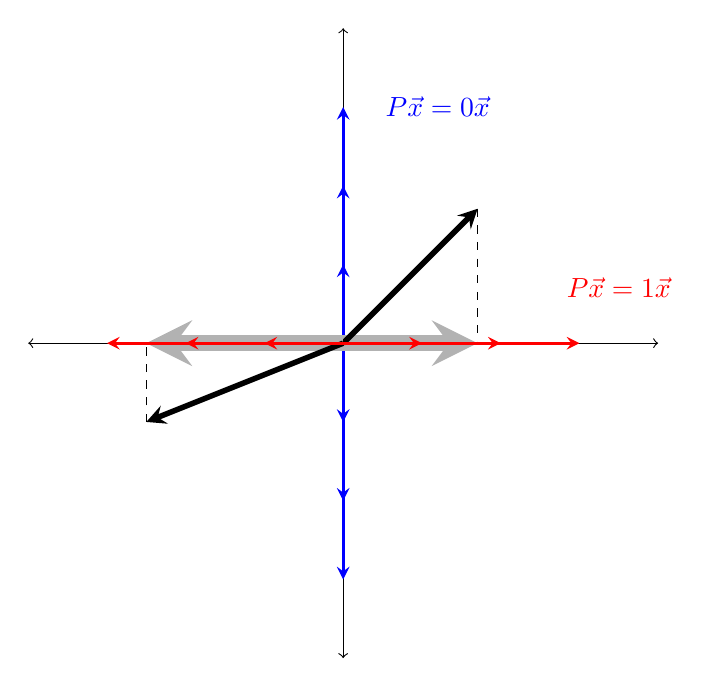
\begin{tikzpicture}
    
    \draw[<->] (-4,0)--(4,0);
    \draw[<->] (0,-4)--(0,4);
    
    \draw[line width=1pt,-stealth, blue](0, 0)--(0, 1);
    \draw[line width=1pt,-stealth, blue](0, 0)--(0, 2);
    \draw[line width=1pt,-stealth, blue](0, 0)--(0, 3);
    \draw[line width=1pt,-stealth, blue](0, 0)--(0, -1);
    \draw[line width=1pt,-stealth, blue](0, 0)--(0, -2);
    \draw[line width=1pt,-stealth, blue](0, 0)--(0, -3);
    
    
\draw[line width=0.5pt,dashed, black](1.707,1.707)--(1.707,0);
\draw[line width=6pt,-stealth, black!30!white](0,0)--(1.707,0);
\draw[line width=2pt,-stealth, black](0, 0)--(1.707,1.707);
    
    
\draw[line width=0.5pt,dashed, black](-2.5,-1)--(-2.5,0);
\draw[line width=6pt,-stealth, black!30!white](0,0)--(-2.5,0);
\draw[line width=2pt,-stealth, black](0, 0)--(-2.5,-1);
    
\draw[line width=1pt,-stealth, red](0, 0)--(-3,0);
\draw[line width=1pt,-stealth, red](0, 0)--(-2,0);
\draw[line width=1pt,-stealth, red](0, 0)--(-1,0);
\draw[line width=1pt,-stealth, red](0, 0)--(3,0);
\draw[line width=1pt,-stealth, red](0, 0)--(2,0);
\draw[line width=1pt,-stealth, red](0, 0)--(1,0);
    
    
    \node[red] at (3.5, 0.7)   (a) {$P\vec{x}=1\vec{x}$};
    
    \node[blue] at (1.2, 3)   (a) {$P\vec{x}=0\vec{x}$};
    
    %\node[black] at (2.2, -1)   (a) {$\begin{bmatrix}1&0\\0&0\end{bmatrix}\begin{bmatrix}x_1\\x_2\end{bmatrix}=\begin{bmatrix}x_1\\0\end{bmatrix}$};
    \end{tikzpicture}
\end{center}
    
The blue vectors along the y-axis are also eigenvectors.  To see this, note that each of the blue vectors is of the form $\vec{x}=\begin{bmatrix}0\\x_2\end{bmatrix}$.  But then $$P\vec{x}=\begin{bmatrix}1&0\\0&0\end{bmatrix}\begin{bmatrix}0\\x_2\end{bmatrix}=\begin{bmatrix}0\\0\end{bmatrix}=0\begin{bmatrix}0\\x_2\end{bmatrix}=0\vec{x}$$
So each of the blue vectors is an eigenvector of $P$ with the corresponding eigenvalue of $0$.
\end{explanation}
\end{example}
    
\begin{exploration}\label{exp:eigenvectors}
Let $A=\begin{bmatrix}1&6\\1&0\end{bmatrix}$.  Again interact with the GeoGebra Applet, for this matrix, to view the scaling of its eigenvectors according to eigenvalues. Return to Standard Basis as needed to set vectors $\vec{v}$ to integer values.
    
    
\begin{center}
    \geogebra{fxktu8e2}{1073}{592}
\end{center}
    
\begin{question}
Note that vectors $\vec{x}_1=\begin{bmatrix}3\\1\end{bmatrix}$ and $\vec{x}_2=\begin{bmatrix}-2\\1\end{bmatrix}$ (and their scalar multiples) remain positioned along the same lines even as they change magnitude and direction.  This indicates that $\vec{x}_1$ and $\vec{x}_2$, along with all of their scalar multiples, are eigenvectors of $A$.  What are the eigenvalues associated with these eigenvectors?
    
Eigenvalue associated with $\vec{x}_1$ is $\lambda_1=\answer{3}$.
    
Eigenvalue associated with $\vec{x}_2$ is $\lambda_2=\answer{-2}$.
    
\begin{hint}
    The interactive shows the result of multiplication by $A$.
    Consider one eigenvector at a time.  Multiplication by what scalar would yield the same result?
\end{hint}
\end{question}
\end{exploration}
    
    
A natural question is this: does every square matrix have eigenvalues and eigenvectors?  We will see later that the answer to this question is ``yes", provided that we permit eigenvalues and entries of eigenvectors to be complex numbers.  The next example is one that requires complex numbers.
    
\begin{example}\label{ex:eigsrotation}
Let $M=\begin{bmatrix}
\frac{\sqrt{2}}{2} & -\frac{\sqrt{2}}{2}\\
\frac{\sqrt{2}}{2} & \frac{\sqrt{2}}{2}
\end{bmatrix}$.  Note that $M$ takes any vector $\vec{x}$ in $\RR^2$ and rotates it by $\frac{\pi}{4}$ radians. 
    
\begin{center}
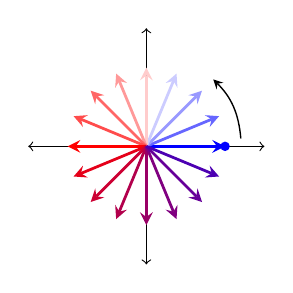
\begin{tikzpicture}
    
    \draw[<->] (-1.5,0)--(1.5,0);
    \draw[<->] (0,-1.5)--(0,1.5);
    
    \draw[line width=1pt,-stealth, blue](0, 0)--(1,0);
    \draw[line width=1pt,-stealth, blue!60!white](0, 0)--(0.924,0.383);
    \draw[line width=1pt,-stealth, blue!40!white](0, 0)--(0.707,0.707);
    \draw[line width=1pt,-stealth, blue!20!white](0, 0)--(0.383,0.924);
    \draw[line width=1pt,-stealth, red!20!white](0, 0)--(0,1);
    
    \draw[line width=1pt,-stealth, red!40!white](0, 0)--(-0.383,0.924);
\draw[line width=1pt,-stealth, red!60!white](0, 0)--(-0.707,0.707);
\draw[line width=1pt,-stealth, red!70!white](0, 0)--(-0.924, 0.383);
\draw[line width=1pt,-stealth, red](0, 0)--(-1,0);
    
\draw[line width=1pt,-stealth, red!90!blue](0, 0)--(-0.924,-0.383);
\draw[line width=1pt,-stealth, red!80!blue](0, 0)--(-0.707,-0.707);
\draw[line width=1pt,-stealth, red!70!blue](0, 0)--(-0.383,-0.924);
\draw[line width=1pt,-stealth, red!60!blue](0, 0)--(0,-1);
    
\draw[line width=1pt,-stealth, red!50!blue](0, 0)--(0.383,-0.924);
\draw[line width=1pt,-stealth, red!40!blue](0, 0)--(0.707,-0.707);
\draw[line width=1pt,-stealth, red!30!blue](0, 0)--(0.924,-0.383);
\fill[blue] (1,0) circle (0.06cm);
    
\draw [->,line width=0.5pt,-stealth]  (1.2,0.1) to[out=95, in=-45] (0.85, 0.85);
    \end{tikzpicture}
    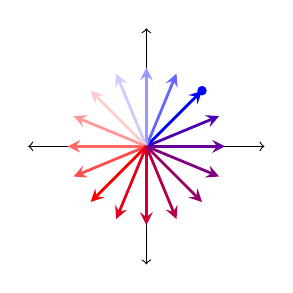
\begin{tikzpicture}
    \draw[<->] (-1.5,0)--(1.5,0);
    \draw[<->] (0,-1.5)--(0,1.5);
    
    \draw[line width=1pt,-stealth, red!40!blue](0, 0)--(1,0);
    \draw[line width=1pt,-stealth, red!30!blue](0, 0)--(0.924,0.383);
    \draw[line width=1pt,-stealth, blue](0, 0)--(0.707,0.707);
    \draw[line width=1pt,-stealth, blue!60!white](0, 0)--(0.383,0.924);
    \draw[line width=1pt,-stealth, blue!40!white](0, 0)--(0,1);
    
    \draw[line width=1pt,-stealth, blue!20!white](0, 0)--(-0.383,0.924);
\draw[line width=1pt,-stealth, red!20!white](0, 0)--(-0.707,0.707);
\draw[line width=1pt,-stealth, red!40!white](0, 0)--(-0.924, 0.383);
\draw[line width=1pt,-stealth, red!60!white](0, 0)--(-1,0);
    
\draw[line width=1pt,-stealth, red!70!white](0, 0)--(-0.924,-0.383);
\draw[line width=1pt,-stealth, red](0, 0)--(-0.707,-0.707);
\draw[line width=1pt,-stealth, red!90!blue](0, 0)--(-0.383,-0.924);
\draw[line width=1pt,-stealth, red!80!blue](0, 0)--(0,-1);
    
\draw[line width=1pt,-stealth, red!70!blue](0, 0)--(0.383,-0.924);
\draw[line width=1pt,-stealth, red!60!blue](0, 0)--(0.707,-0.707);
\draw[line width=1pt,-stealth, red!50!blue](0, 0)--(0.924,-0.383);
    
\fill[blue] (0.707,0.707) circle (0.06cm);
    \end{tikzpicture}
\end{center}
    
    
    
%{\color{red} Inserting a tikz here would be nice, I think.}
    
Since $M$ rotates every vector in $\RR^2$, \wordChoice{\choice[correct]{every}\choice{some}\choice{no}} nonzero vector(s) changes direction, so there \wordChoice{\choice{are}\choice[correct]{are no}} eigenvectors in the plane.  

It turns out that $M$ does have eigenvectors and eigenvalues, but in order to find them we need to work with vectors whose entries are complex numbers. As a brief review, complex numbers are numbers of the form $a+bi$, where $a$ and $b$ are real numbers and $i$ is the imaginary unit, which is defined to be $i=\sqrt{-1}$. The real part of $a+bi$ is $a$, and the complex part of $a+bi$ is $b$. Any complex numbers with complex parts are not visible in the plane, so we cannot see the eigenvectors of $M$.  
    
To follow the computation below, you need to recall that the imaginary unit $i$ is defined to by $i^2=-1$, and that for two complex numbers $a+bi$ and $c+di$, their product is computed as follows:
$$(a+bi)(c+di)=ac+adi+bci+bdi^2=ac+adi+bci-bd=(ac-bd)+i(ad+bc)$$
    
    
%\begin{center}[3in]
%\begin{tikzpicture}
    
    % \draw[<->] (-4,0)--(4,0);
    % \draw[<->] (0,-4)--(0,4);
    
% \node[blue] at (0, 2)   (a) {Eigenvectors? What eigenvectors?  Nothing to see here...};
    
% \end{tikzpicture}
%\end{center}
    
%{\color{blue}I was just being goofy, do we seriously want to keep this?}
    
Consider the vector $\begin{bmatrix} \frac{\sqrt{2}}{2}\\ \frac{\sqrt{2}}{2} i \end{bmatrix}$.  We compute:
$$\begin{bmatrix}
\frac{\sqrt{2}}{2} & -\frac{\sqrt{2}}{2}\\
\frac{\sqrt{2}}{2} & \frac{\sqrt{2}}{2}
\end{bmatrix} \begin{bmatrix} \frac{\sqrt{2}}{2}\\ \frac{\sqrt{2}}{2} i \end{bmatrix} =
\begin{bmatrix} \frac{1}{2}-\frac{1}{2} i\\ \frac{1}{2}+ \frac{1}{2} i \end{bmatrix}= (\frac{\sqrt{2}}{2}-\frac{\sqrt{2}}{2}i) \begin{bmatrix} \frac{\sqrt{2}}{2}\\ \frac{\sqrt{2}}{2} i \end{bmatrix},$$
so \(\begin{bmatrix} \answer{\frac{\sqrt{2}}{2}}\\ \answer{\frac{\sqrt{2}}{2}}i \end{bmatrix}\) is an eigenvector of \(M\). Its corresponding eigenvalue is \(\answer{\frac{\sqrt{2}}{2}-\frac{\sqrt{2}}{2}i}\). (just type ``i'' for the imaginary unit).
\end{example}
    
We will continue to work with complex numbers as we study eigenvalues and eigenvectors.
    
\subsection*{Why All the Fuss About Eigenvalues and Eigenvectors?}
    
\begin{remark}
The first in-depth study of eigenvalues can probably be attributed to Fourier as he studied partial differential equations early in the nineteenth century, and in particular when he studied what is known as the heat equation. [Trefethen and  Embree]  By the twentieth century mathematicians understood the connections between differential equations and eigenvalues. Systems of differential equations are often best represented by matrices, especially in the context of using computers to find numerical solutions. Most algorithms to solve these systems work by iterating some process, and eigenvalues along with their corresponding eigenvectors indicate what will happen to such a process after many repetitions.
    
The most famous modern example of a large-scale eigenvalue problem is the Google PageRank algorithm, which helped set Google apart from its competitors as a search engine.  Some of the relevant mathematics can be learned by working through the paper, \href{https://doi.org/10.1137/050623280}{``The \$25,000,000,000 Eigenvector, The Linear Algebra Behind Google''}, by Kurt Bryan and Tanya Leise. 
\end{remark}

    
\section*{Bibliography}
[Trefethen and  Embree] Trefethen, Lloyd and Embree, Mark, {\it Spectra and Pseudospectra}, Princeton University Press, 2005, p. 5-6


\end{document}